
\begin{frame}[c]{Modell der Selbstmanagement-Kompetenz}
    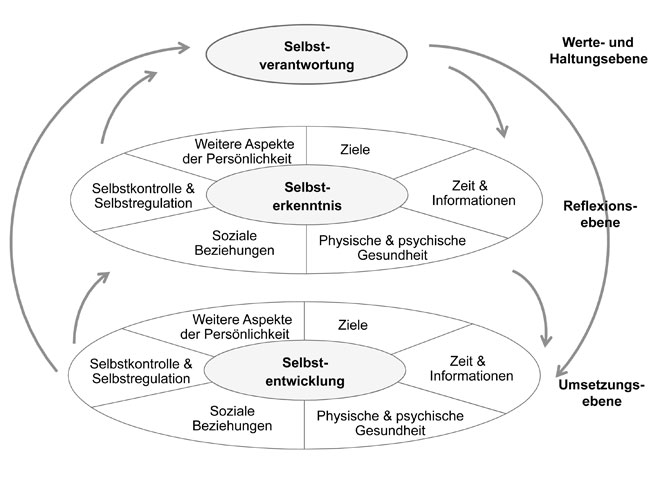
\includegraphics[width=\textwidth]{zsm/modell.jpeg}
\end{frame}


\section{Selbstverantwortung}

\begin{frame}[c]{Selbstverantwortung - Verhaltensindikatoren}
    \begin{itemize}
    \item Persönliche Lebensphilosophie
    \pause
    \item Verantwortung für eigenes Leben und Lebensführung übernehmen
    \pause
    \item Schuld für Missstände nicht externalisieren
    \pause
    \item Sich über Selbst- und Fremdbestimmung bewusst sein
    \end{itemize}
\end{frame}


\begin{frame}[c]{Selbstverantwortung - Reflektionsfragen}
    \begin{itemize}
    \item Was ist mir im Leben am wichtigsten? \newline
    \pause
    \item Wirkt sich Fremdbestimmung Negativ auf mein Wohlbefinden aus? \newline
    \pause
    \item Überneheme ich genug Verantwortung für mein Wohlbefinden?
    \end{itemize}
\end{frame}


\begin{frame}[standout]
    Was Wünsche ich mir für meine Zukunft?
\end{frame}





\section{Selbsterkenntnis}

\begin{frame}[c]{Selbsterkenntnis - Verhaltensindikatoren}
    \begin{itemize}
    \item Erkenntnisgewinn über das eigene Selbst (Realistische Reflektion) \newline
    \pause
    \item Bewusstsein für das eigene Verhalten entwickeln \newline
    \pause
    \item Erkennen und akzeptieren eigener Schwächen \newline
    \end{itemize}
\end{frame}


\begin{frame}[c]{Selbsterkenntnis - Reflektionsfragen}
    \begin{itemize}
    \item Was sagt mir mein Körper wie es mir geht? \newline
    \pause
    \item Was kann ich gut? \newline
    \pause
    \item Welche Einstellungen und Verhaltensmuster Prägen mich?
    \end{itemize}
\end{frame}


\begin{frame}[c]{Selbsterkenntnis - Übung}
    
\end{frame}





\section{Selbstentwicklung}

\begin{frame}[c]{Selbstentwicklung - Verhaltensindikatoren}
    \begin{itemize}
    \item Weiterentwicklung der Persönlichkeit mit dem verlauf des Lebens
    \pause
    \item Klares hinarbeiten auf eigen Ziele
    \pause
    \item Offenheit neuen Erfahrungen gegenüber erhalten
    \pause
    \item Eigene Einstellung verändern können
    \end{itemize}
\end{frame}


\begin{frame}[c]{Selbstentwicklung - Reflektionsfragen}
    \begin{itemize}
    \item Was will ich im Leben noch Erfahren/Lernen/Wissen? \newline
    \pause
    \item Wo schränke ich mich in meinen Möglichkeiten selbst ein? \newline
    \pause
    \item Wie ist meine Körperhaltung jetzt gerade?
    \end{itemize}
\end{frame}


\begin{frame}[c]{Selbstentwicklung - Übung}
    
\end{frame}





\section{Ziele}

\begin{frame}[c]{Ziele - Anwendung}
    \begin{itemize}
    \item Persönliche Ziele Definieren und Analysieren\pause Wichtig: Realisierbarkeit
    \pause
    \item Zielkonflikte erkennen und behandeln
    \pause
    \item Konkrete Handlungspläne für die Zielerreichung umfassend ausgestalten
    \pause
    \item Entschlossen an Zielen festhalten
    \end{itemize}
\end{frame}





\section{Zeit und Informationen}

\begin{frame}[c]{Zeitmanagement}
    \begin{itemize}
    \item Zeit bewusst und zielorientiert einteilen
    \pause
    \item Erholung gezielt in den Zeitplan integrieren
    \pause
    \item Zeitdiebe Elimieren
    \pause
    \item Differenzieren zwischen nützlichen und hinderlichen Aktivitäten
    \end{itemize}
\end{frame}



\section{Physische und Psychische Gesundheit}

\begin{frame}[c]{Gesundheit}
    \begin{itemize}
    \item Bewusstsein für die Wichtigkeit des eigenen Physischen und Psychischen Zustands entwickeln
    \pause
    \item Balance auf Körperlicher Ebene: \pause Schlaf\pause, Gesunde ernährung\pause, Erholung\pause, Bewegung
    \pause
    \item Balance auf Emotionaler Ebene: \pause Emotionsmanagement\pause, Erregungskontrolle
    \end{itemize}
\end{frame}



\section{Soziale Beziehungen}

\begin{frame}[c]
    
\end{frame}



\section{Selbstkontrolle und Selbstrugalation}




\section{Relevante Aspekte der Persönlichkeit}



























